\documentclass{article}

\usepackage{tikz}
\usepackage{amsmath}
\usepackage[left=2.3cm, right=2.3cm, top=1.7cm, bottom=1.7cm]{geometry}

\usepackage{Sweave}
\begin{document}
\input{test-concordance}

{\Large \textbf{Name:}} \hspace{3cm} \vspace{1cm}


\begin{center}
{\Huge Stage 1 - General Mathematics Networks Test}
\end{center}

\vspace{0.6cm}
\begin{center}
{\Large \emph{\textbf{Express all answers with positive indices.}}}
\end{center}
\vspace{0.2cm}

{\Large \textbf{Question 1} Simplify \\[6pt]
\textbf{(a)} {\Large $h^2 \times h^3$} \hfill \textbf{(b)} {\huge $\frac{b^7}{b^4}$} \hfill \textbf{(c)} {\Large $g^8 \times g^{-2}$}}

\vspace{0.1cm}
\begin{center}

\begin{tikzpicture}
\draw[step=0.5,black,thin] (0,0) grid (16, 7);
\end{tikzpicture}
\end{center}
\vspace{0.6cm}

{\Large \textbf{Question 2} Evaluate \\[6pt]
\textbf{(a)} {\Large $2^3 \times 5^3$} \hfill \textbf{(b)} {\Large $(32)^{0.2}$} \hfill \textbf{(c)} {\Large $3 \times 5^{-2}$}}

\vspace{0.1cm}
\begin{center}

\begin{tikzpicture}
\draw[step=0.5,black,thin] (0,0) grid (16, 7);
\end{tikzpicture}
\end{center}

\pagebreak
{\Large \textbf{Question 3} Simplify \\[6pt]
\textbf{(a)} {\Large $(2a^{-2})^5$} \hfill \textbf{(b)} {\Large $4g^3h^2 \times 3g^5h^4$} \hfill \textbf{(c)} {\huge $\frac{-36p^7t^4}{-9p^{11}t^{2}}$}}

\vspace{0.1cm}
\begin{center}

\begin{tikzpicture}
\draw[step=0.5,black,thin] (0,0) grid (16, 7);
\end{tikzpicture}
\end{center}

{\Large \textbf{Question 4} Simplify \\[6pt]
\textbf{(a)} {\Large $(2a^{-4}b^3)^3$} \hfill \textbf{(b)} {\huge $\left ( \frac{a^{-5}b}{c^{-3}} \right )^2$} \hfill \textbf{(c)} {\huge $a^{\frac{3}{4}}a^{\frac{2}{3}}$}} 

\vspace{0.1cm}
\begin{center}

\begin{tikzpicture}
\draw[step=0.5,black,thin] (0,0) grid (16, 7);
\end{tikzpicture}
\end{center}


\pagebreak
{\Large \textbf{Question 5} \\[-6pt]

\begin{center}
\includegraphics{./fractal.png}
\end{center}

The above shows how a fractal is constructed  in stages from left to right. Each stage is constructed from the previous stage by splitting each remaining square into 9 equal squares and removing 4 of them. Stage 0 (the leftmost image) is a $1 \times 1$ square, so it has total area of 1 $\text{unit}^2$.
\vspace{0.4cm}

\textbf{(a)} Explain why stage 1 has a total area of {\huge $\frac{5}{9}$} $\text{unit}^2$.

\vspace{0.4cm}
\begin{center}
\begin{tikzpicture}[scale=0.8]
\draw[black,thin] (0,0) -- (20, 0);
\draw[black,thin] (0,1) -- (20, 1);
\draw[black,thin] (0,2) -- (20, 2);
\draw[black,thin] (0,3) -- (20, 3);
\draw[black,thin] (0,4) -- (20, 4);
\draw[black,thin] (0,5) -- (20, 5);
\draw[black,thin] (0,6) -- (20, 6);
\end{tikzpicture}
\end{center}
\vspace{0.2cm}

\textbf{(b)} Explain why stage 2 has a total area of {\huge $\frac{25}{81}$} $\text{unit}^2$.

\vspace{0.4cm}
\begin{center}
\begin{tikzpicture}[scale=0.8]
\draw[black,thin] (0,0) -- (20, 0);
\draw[black,thin] (0,1) -- (20, 1);
\draw[black,thin] (0,2) -- (20, 2);
\draw[black,thin] (0,3) -- (20, 3);
\draw[black,thin] (0,4) -- (20, 4);
\draw[black,thin] (0,5) -- (20, 5);
\draw[black,thin] (0,6) -- (20, 6);
\end{tikzpicture}
\end{center}
\vspace{0.2cm}


\pagebreak 

{\Large \textbf{Question 5 continued...} \\[6pt]

\textbf{(c)} Write {\huge $\frac{25}{81}$} as a power of {\huge $\frac{5}{9}$}

\vspace{0.1cm}
\begin{center}
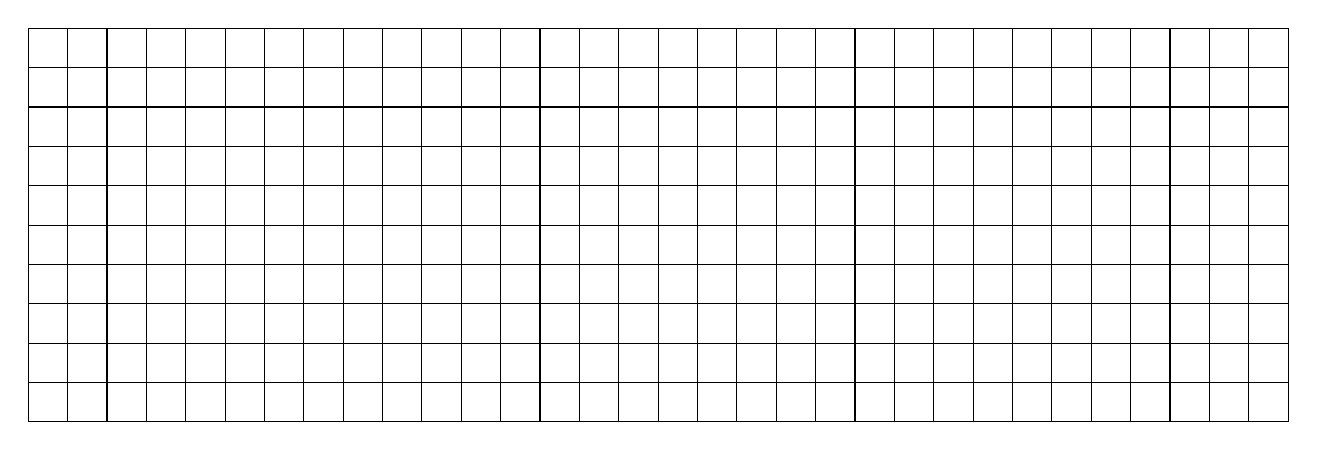
\begin{tikzpicture}
\draw[step=0.5,black,thin] (0,0) grid (16, 5);
\end{tikzpicture}
\end{center}

\textbf{(d)} Write an expression \emph{using indices} to represent the area of Stage 3.

\vspace{0.1cm}
\begin{center}
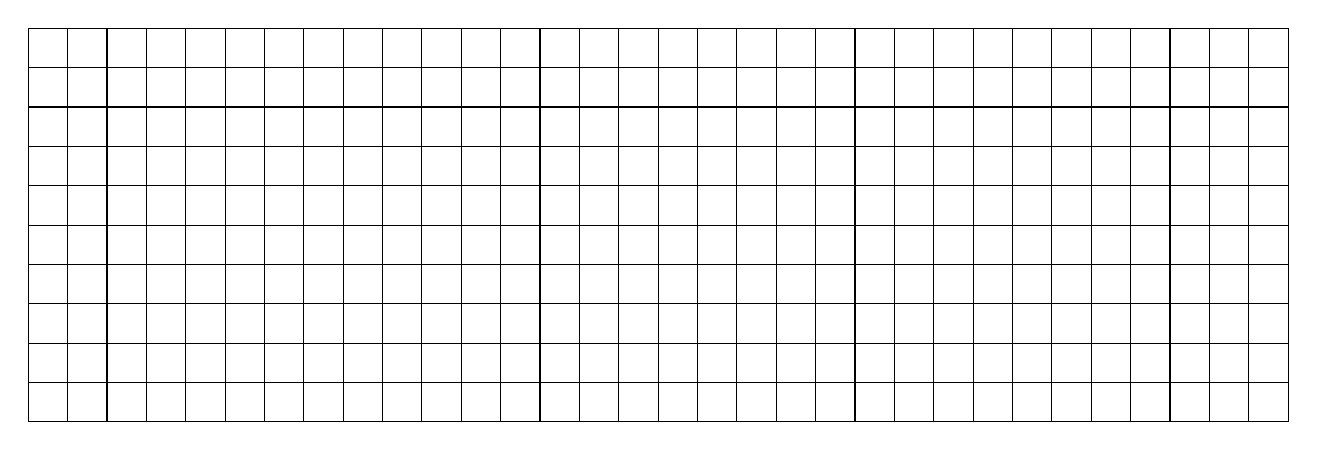
\begin{tikzpicture}
\draw[step=0.5,black,thin] (0,0) grid (16, 5);
\end{tikzpicture}
\end{center}

\textbf{(e)} Hence, or otherwise, write an expression \emph{using indices} to represent the area of Stage $n$.

\vspace{0.1cm}
\begin{center}
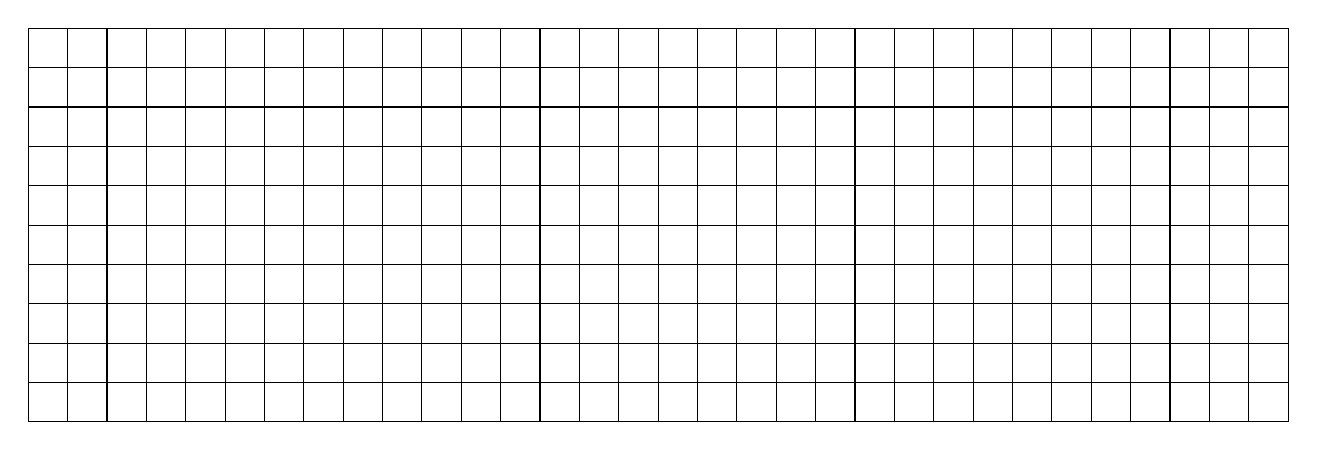
\begin{tikzpicture}
\draw[step=0.5,black,thin] (0,0) grid (16, 5);
\end{tikzpicture}
\end{center}






\end{document}
